\chapter{Orderbook Trading Simulator}
\label{chap:simulator}
This chapter describes the \ac{OTS} and it's underlying OrderbookContainers, implemented within the scope of this thesis. Fed with historic orderbook data it serves as a backtesting framework for testing out various trading strategies. The \ac{OTS} provides detailed feedback in terms of trading progress, achieved prices and accrued costs.

\section{Data Origin}
Since typical financial data providers must make an earning from their treasures, they typically only deliver delayed market data on a complimentary basis. Investors dependent on real time or level 2 market data (see \Cref{sec:marketdata:levels}) are usually charged horrendous monthly subscription fees.\\

A costless alternative exists in open cryptocurrencies, like bitcoins (see \Cref{chap:bitcoins}). The digital asset exchange platform Poloniex \cite{poloniex} provides an open API for querying detailed market data in real time. As their push API, to receive live order book updates and trades, was rather error-prone and buggy when this project started, the decision was made, to query full orderbooks on a minutely basis.\\

On Nov, 10th 2016, 10:00 am, a daemon was started, to fetch orderbook snapshots up to a market depth of 5000 from Poloniex via HTTP GET requests. The volume of recorded orderbook snapshots for nine distinct currency pairs\footnote{Recorded currency pairs include USDT/BTC, BTC/ETH, BT/XMR, BTC/XRP, BTC/FCT, BTC/NAV, BTC/DASH, BTC/MAID, BTC/ZEC} has since grown to roughly 100GB (as per 2017-06-20). This thesis is based on a condensed version of the currency pair USDT/Bitcoin.

\begin{lstlisting}[frame=single, breaklines=true, basicstyle=\scriptsize, caption=Data fetched from Poloniex via HTTP GET request, label=lst:PoloniexFetch]
# https://poloniex.com/public?command=returnOrderBook&currencyPair=USDT_BTC&depth=5000
{"asks" :[[ "705.450000" ,2.772181], [ "705.450196", 0.139212] ,["706.170000" ,0.052838] , ... ], "bids":[["705.000000",0.158232],["703.700000" ,0.001250], ... ], "isFrozen": 0, "seq": 63413296}
\end{lstlisting}

\begin{figure}[ht]
	\centering
   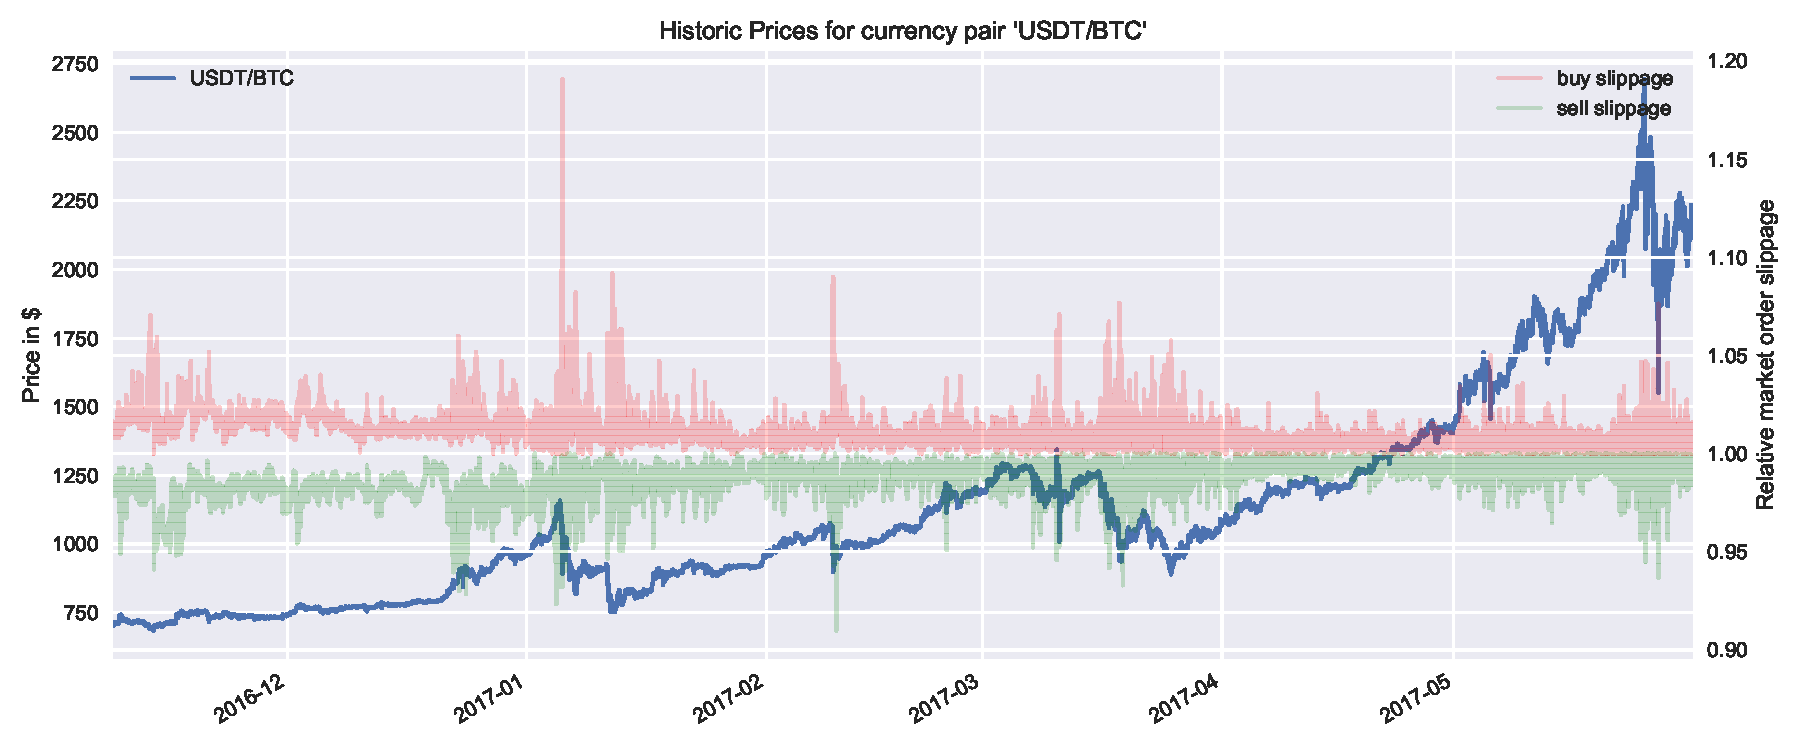
\includegraphics[width=0.7\textwidth]{content/drawings/bitcoin_historicPrices}
	\caption{Historic center prices between Nov, 10th 2016 and Mar, 31 2017, as fetched from Poloniex}
	\label{fig:ploniexPriceHistory}
\end{figure}

\section{Data preprocessing}
\label{chap:preprocessing}
The python \lstinline!class OrderbookContainer! aggregates all informations contained in an individual orderbook snapshot. It enforces correct price ordering in the two opposing bid and ask books and provides additional methods for market visualization and feature extraction. To restrict wasteful memory usage, orderbook snapshots are condensed in two ways:

\begin{itemize}
\item Almost identically price levels are round to the second decimal and their respective order volumes merged.

 \[ 
  \begin{rcases}
    0.139212 * 705.450000\\
    2.632969 * 705.450196\\
  \end{rcases} 
  = 2.772181 * 705.45
\]
\item Market depth is capped just above the threshold of 100 bitcoins, roughly corresponding to a market depth of 100-140 prices levels in both books. This threshold allows to simulate trades up to a market order price of 70.000 \$ at any time throughout the whole recording period.

\item Erroneous orderbook snapshots have been discarded.

\end{itemize}

\Cref{lst:OrderbookContainer} shows the most important functions, provided by the OrderbookContainer class. OrderbookContainer instances are vigorously used by the \ac{OTS}.

\begin{lstlisting}[frame=single, breaklines=true, basicstyle=\scriptsize, caption=OrderbookContainer, label=lst:OrderbookContainer]
ob = OrderbookContainer(timestamp="2016-11-08T10:00",
                        bids=pd.DataFrame([200., 100., 300.],
                        columns=['Amount'], index=[28.7, 28.5, 28]),
                        asks=pd.DataFrame([25., 50., 200.],
                        columns=['Amount'], index=[29., 30., 31.]))
# Available methods
ob.plot(outfile='sample.pdf')  # plt.show or plt.savefig
ob.asks  # pd.DataFrame
ob.bids  # pd.DataFrame
ob.features  # returns a dict of precomputed features
ob.get_bid(), ob.get_ask(), ob.get_center()  # float
ob.get_current_price(volume=100)  # achievable cashflow by market order
ob.get_current_sharecount(cash=70000) # number of shares aquirable by market order
ob.compare_with(other_ob) # returns orderbook deltas used by the OTS
ob.enrich()  # computes Volume, VolumeAcc and norm_Price
ob.head(depth=3)  # returns the orderbook, capped at a market depth of 3
ob.plot()
\end{lstlisting}


\begin{figure}[ht]
	\centering
   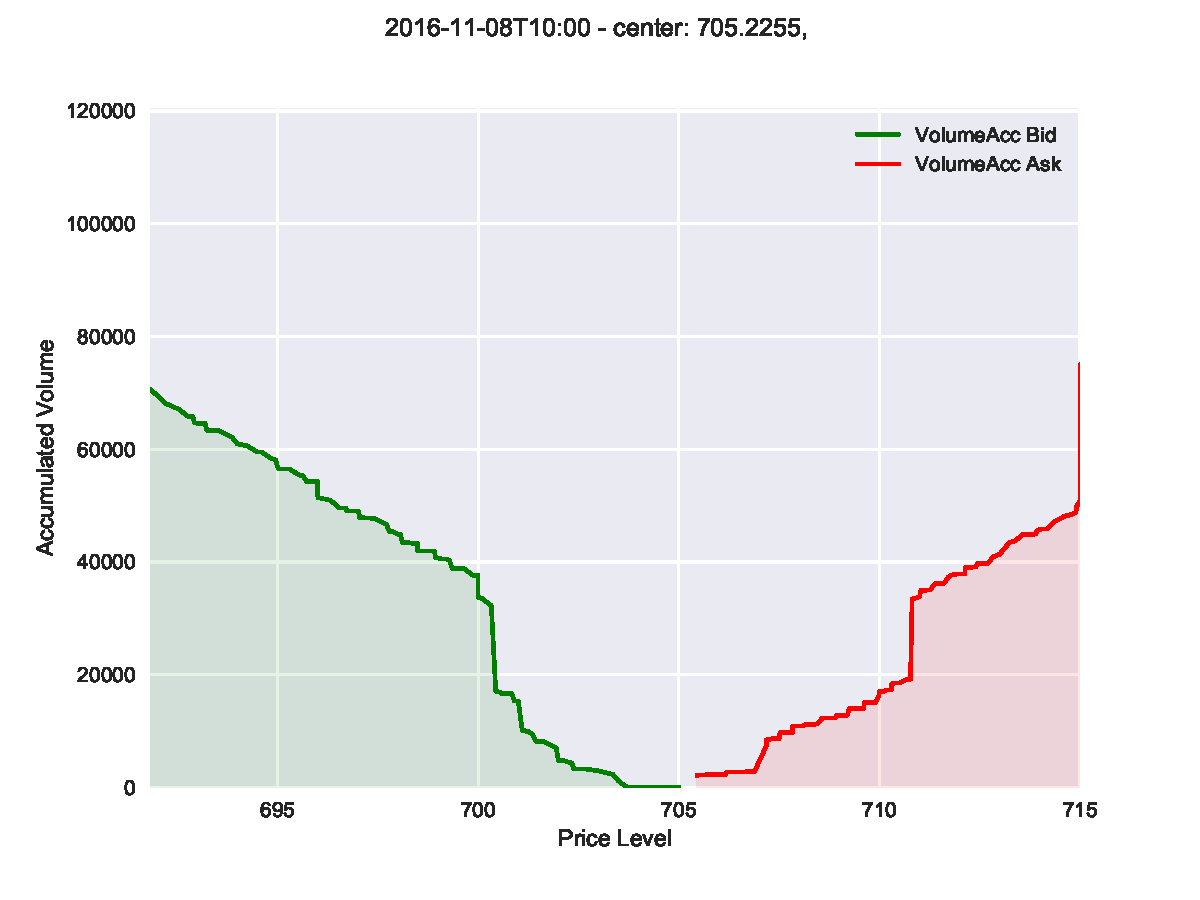
\includegraphics[width=0.9\textwidth]{content/drawings/orderbook}
	\caption{A simple visualization of an limit orderbook.}
	\label{fig:orderbook}
\end{figure}


\section{Simulator}
The \ac{OTS} framework serves as basis for all preceding experiments and evaluations.
Each simulator instance is fed with an array of subsequent OrderbookContainers (\emph{orderbook windows}) and a targeted trading volume $V$, which it pretends to trade into cash or visa versa within a fixed time horizon $H$, according to an external strategy. In the rare case of missing orderbook snapshots (see \Cref{chap:preprocessing}), the \emph{real} time horizon may be larger than usual, since always $H$ subsequent orderbooks are selected.\\

Limit orders may be placed at predefined, discrete time steps within the trading horizon $H$. The simulator is done, once the remaining trading volume is zero, which is enforced at the very last time point. Any remaining volume at \emph{H-1} is transformed into a simple market order and executed immediately, at any price. Additional parameters control the simulators behavior, when its main function \lstinline!trade(limit=...)! is called:

\begin{description}
\item[volume $$] : The targeted trading volume $V$.\\
Positive values indicate buy orders, negative values indicate sell orders.
\item[consume] : \lstinline!'cash'! or \lstinline!'volume'!\\
Defines whether \lstinline!volume! should be interpreted as \emph{cash} (goal: buy/sell shares for $V$ dollars), or as \emph{sharecount} (goal: buy/sell $V$ shares).
\item[period\_length] : \lstinline!default=15!\\
Defines the duration at which a limit order is executed. After a trade has been placed, the simulator iterates over the next \lstinline!period_length! orderbooks, before the results are reported and a reviewed order may be placed.

\item[tradingperiods] : \lstinline!default=4!\\
Defines the number of trade reviews, that can be made within the time horizon $H =$ \lstinline!period_length * tradingperiods!.

\item[costtype] : \lstinline!default='slippage'!\\
Defines which of multiple cost functions to use in the returned reports. 
\end{description}

\Cref{fig:orderbookwindow} visualizes a 60 minutes long orderbook windows, where the solid red lines mark the \emph{average} (a) and \emph{worst} (b) price, that has to be paid at a given time point, in case of an immediate market order of 100, 75, 50 and 25 bitcoins respectively. Analogously, the solid green lines represent achieved prices for sale orders of -25, -50, -75 and -100 bitcoins.\\

As can be seen in this graph, ask prices deviate more from the center price than bid prices. An plausible inference might be, that imbalances between demand and supply might serve as a valuable indicator for future price trends.

\begin{figure}[ht]
	\centering
   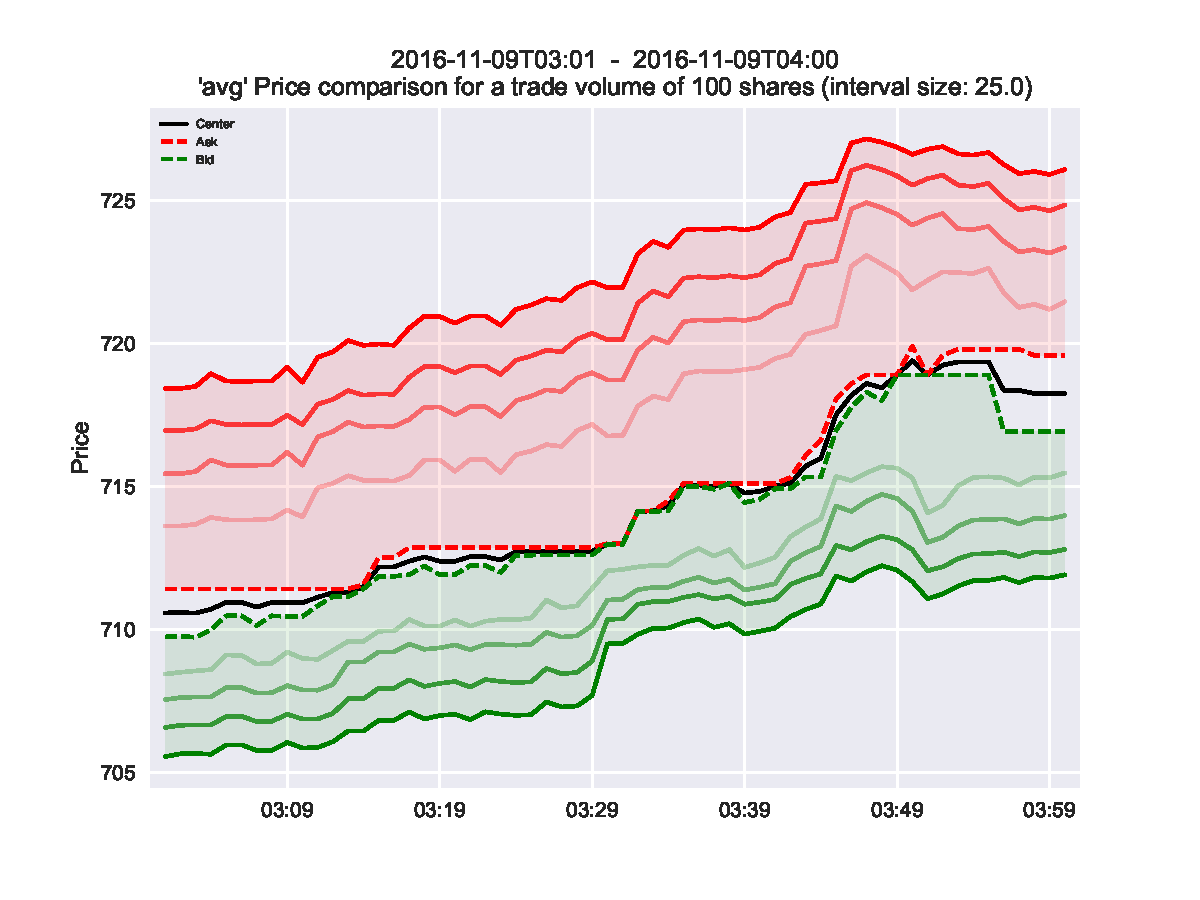
\includegraphics[width=0.49\textwidth]{content/drawings/orderbook_window17} 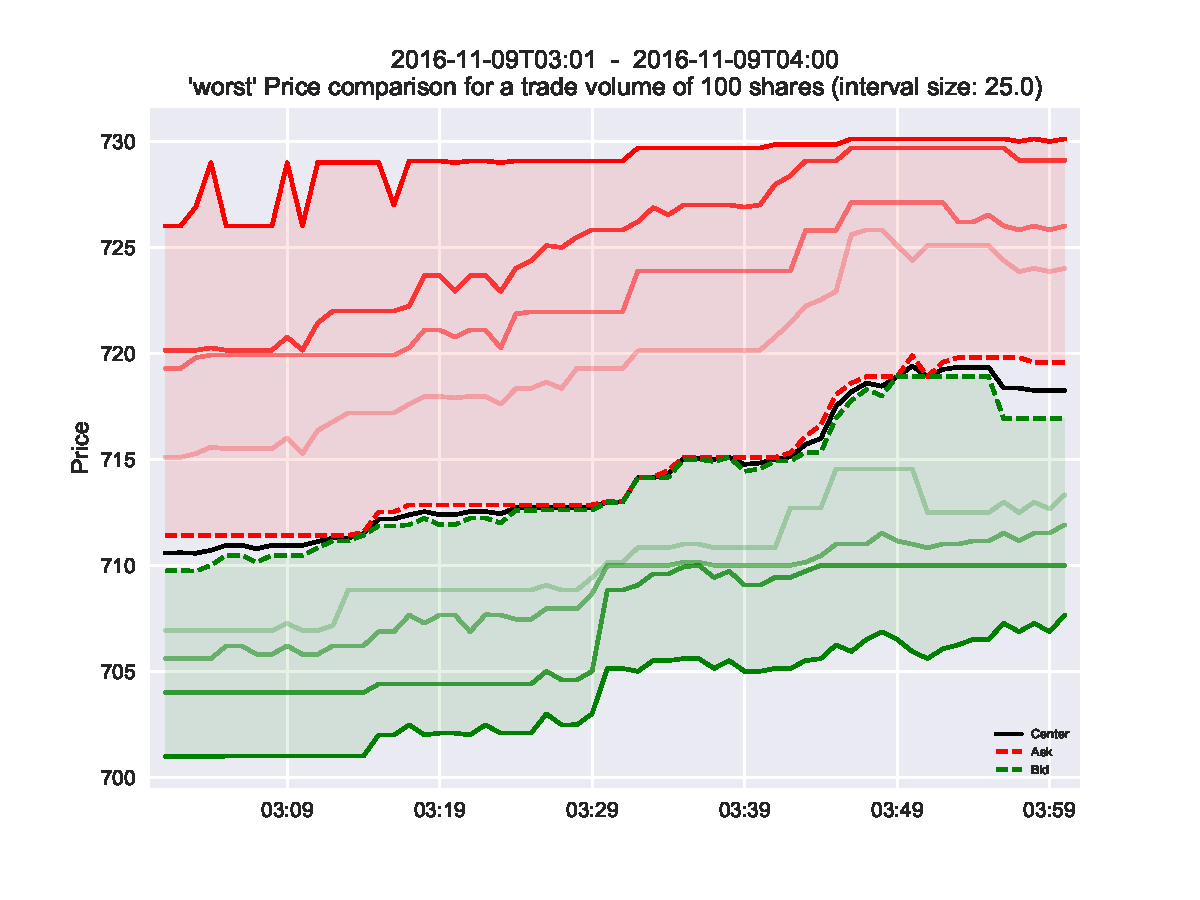
\includegraphics[width=0.49\textwidth]{content/drawings/orderbook_window17_worst}
	\caption{An orderbook window over a period of 60 minutes.}
	\label{fig:orderbookwindow}
\end{figure}

\subsection{Internal Masterbook}
bla

\subsection{Trade execution}
bla

\section{Evaluation / Comparison of strategies}
bla













\cleardoublepage{}